\section{Metodologia}
\subsection{Entorn de proves}
{
    L'entorn de proves s'ha creat amb el software VNX. L'escenari està basat en l'entorn de la pràctica d'IP Multicast
    de l'assignatura de TCGI, ja que és un entorn conegut, ademés de ser suficient per fer la demostració i ser
    lleuger a l'hora de fer modificacions i montar-ho l'ordinador base.

    Totes les màquines virtuals de l'entorn son una rèplica d'un LXC amb el sistema operatiu Ubuntu 18.04 LTS.
    Aquest està provisionat amb tot el software necessari tant pels routers com pels hosts. En el cas de precisar un
    software en desenvolupament, com pot ser els scripts per fer correr el servidor i els clients, llavors
    també es poden copiar al montar l'escenari (VNX permet copiar carpeta especifiques al terminal indicat).

    \begin{figure}[H]
        \label{fig:network}
        \centering
        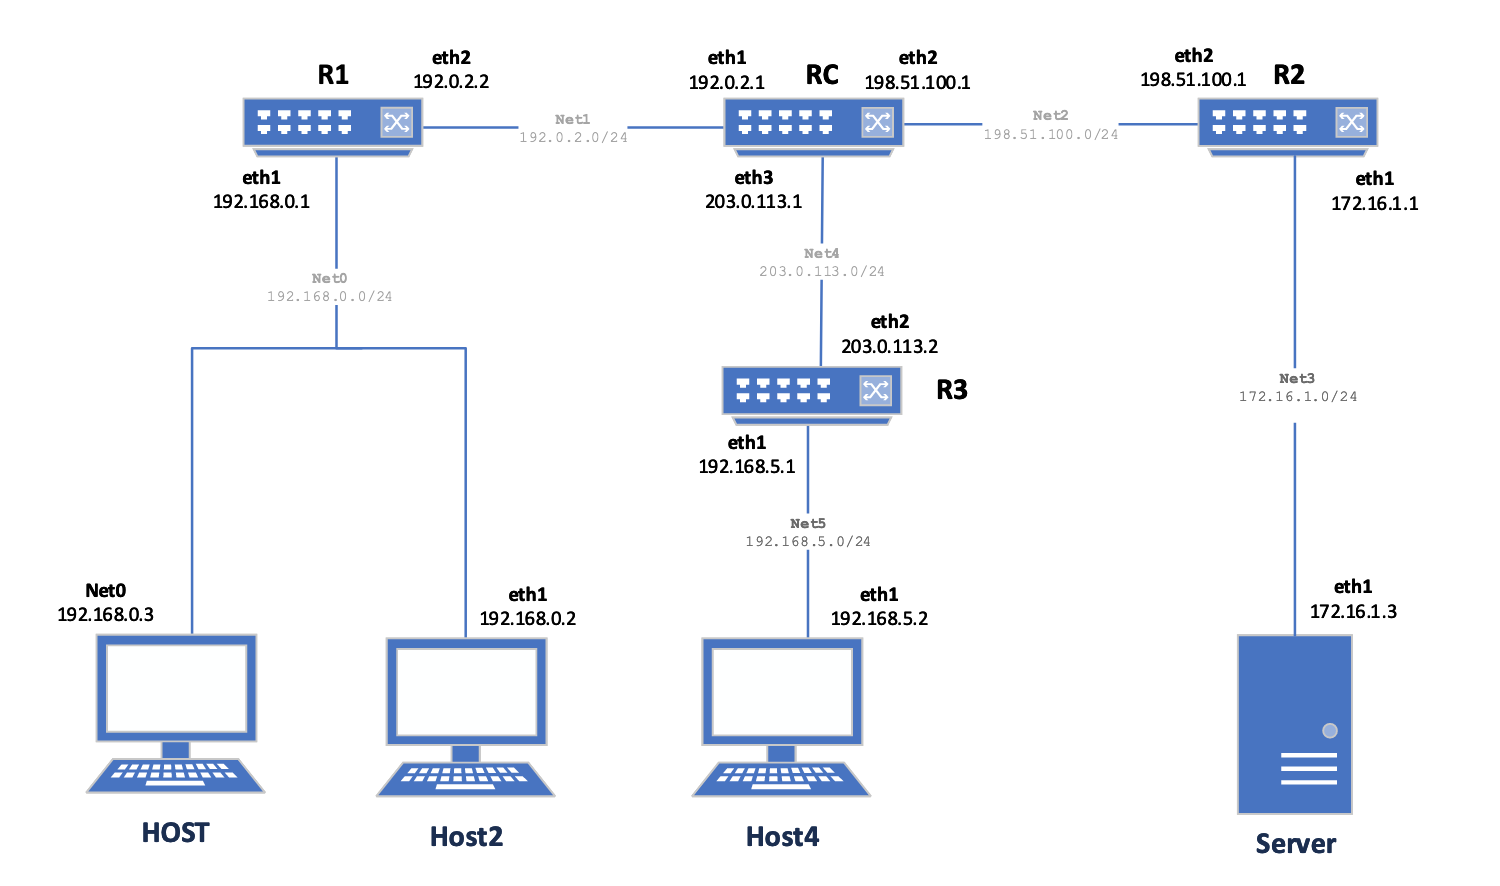
\includegraphics[width=15cm]{img/03_metodologia/network_topology.png}
    \end{figure}

    La topologia de xarxa consisteix en 3 hosts, 2 virtuals i un real (HOST), que rebran la retransmissió;
    4 routers que s'encarreguen de distribuir el contingut segons és necesari; i 1 servidor que emetrà el 
    contingut tant per via multicast com per via unicast.
}

\subsection{Disseny del sistema}
{
    S'ha dissenyat el sistema perquè sigui el més simple possible, fent que l'estructura tant del servidor com
    del client siguin pràcticament semblants tant pel cas unicast com pel cas multicast.De cara a l'usuari final
    s'ha volgut que l'utilització del servidor unicast o del multicast sigui pràcticament igual; és dir, que 
    sigui igual utilitzar un o l'altre a nivell d'\ac{API}. 

    \begin{figure}[H]
        \label{fig:system}
        \centering
        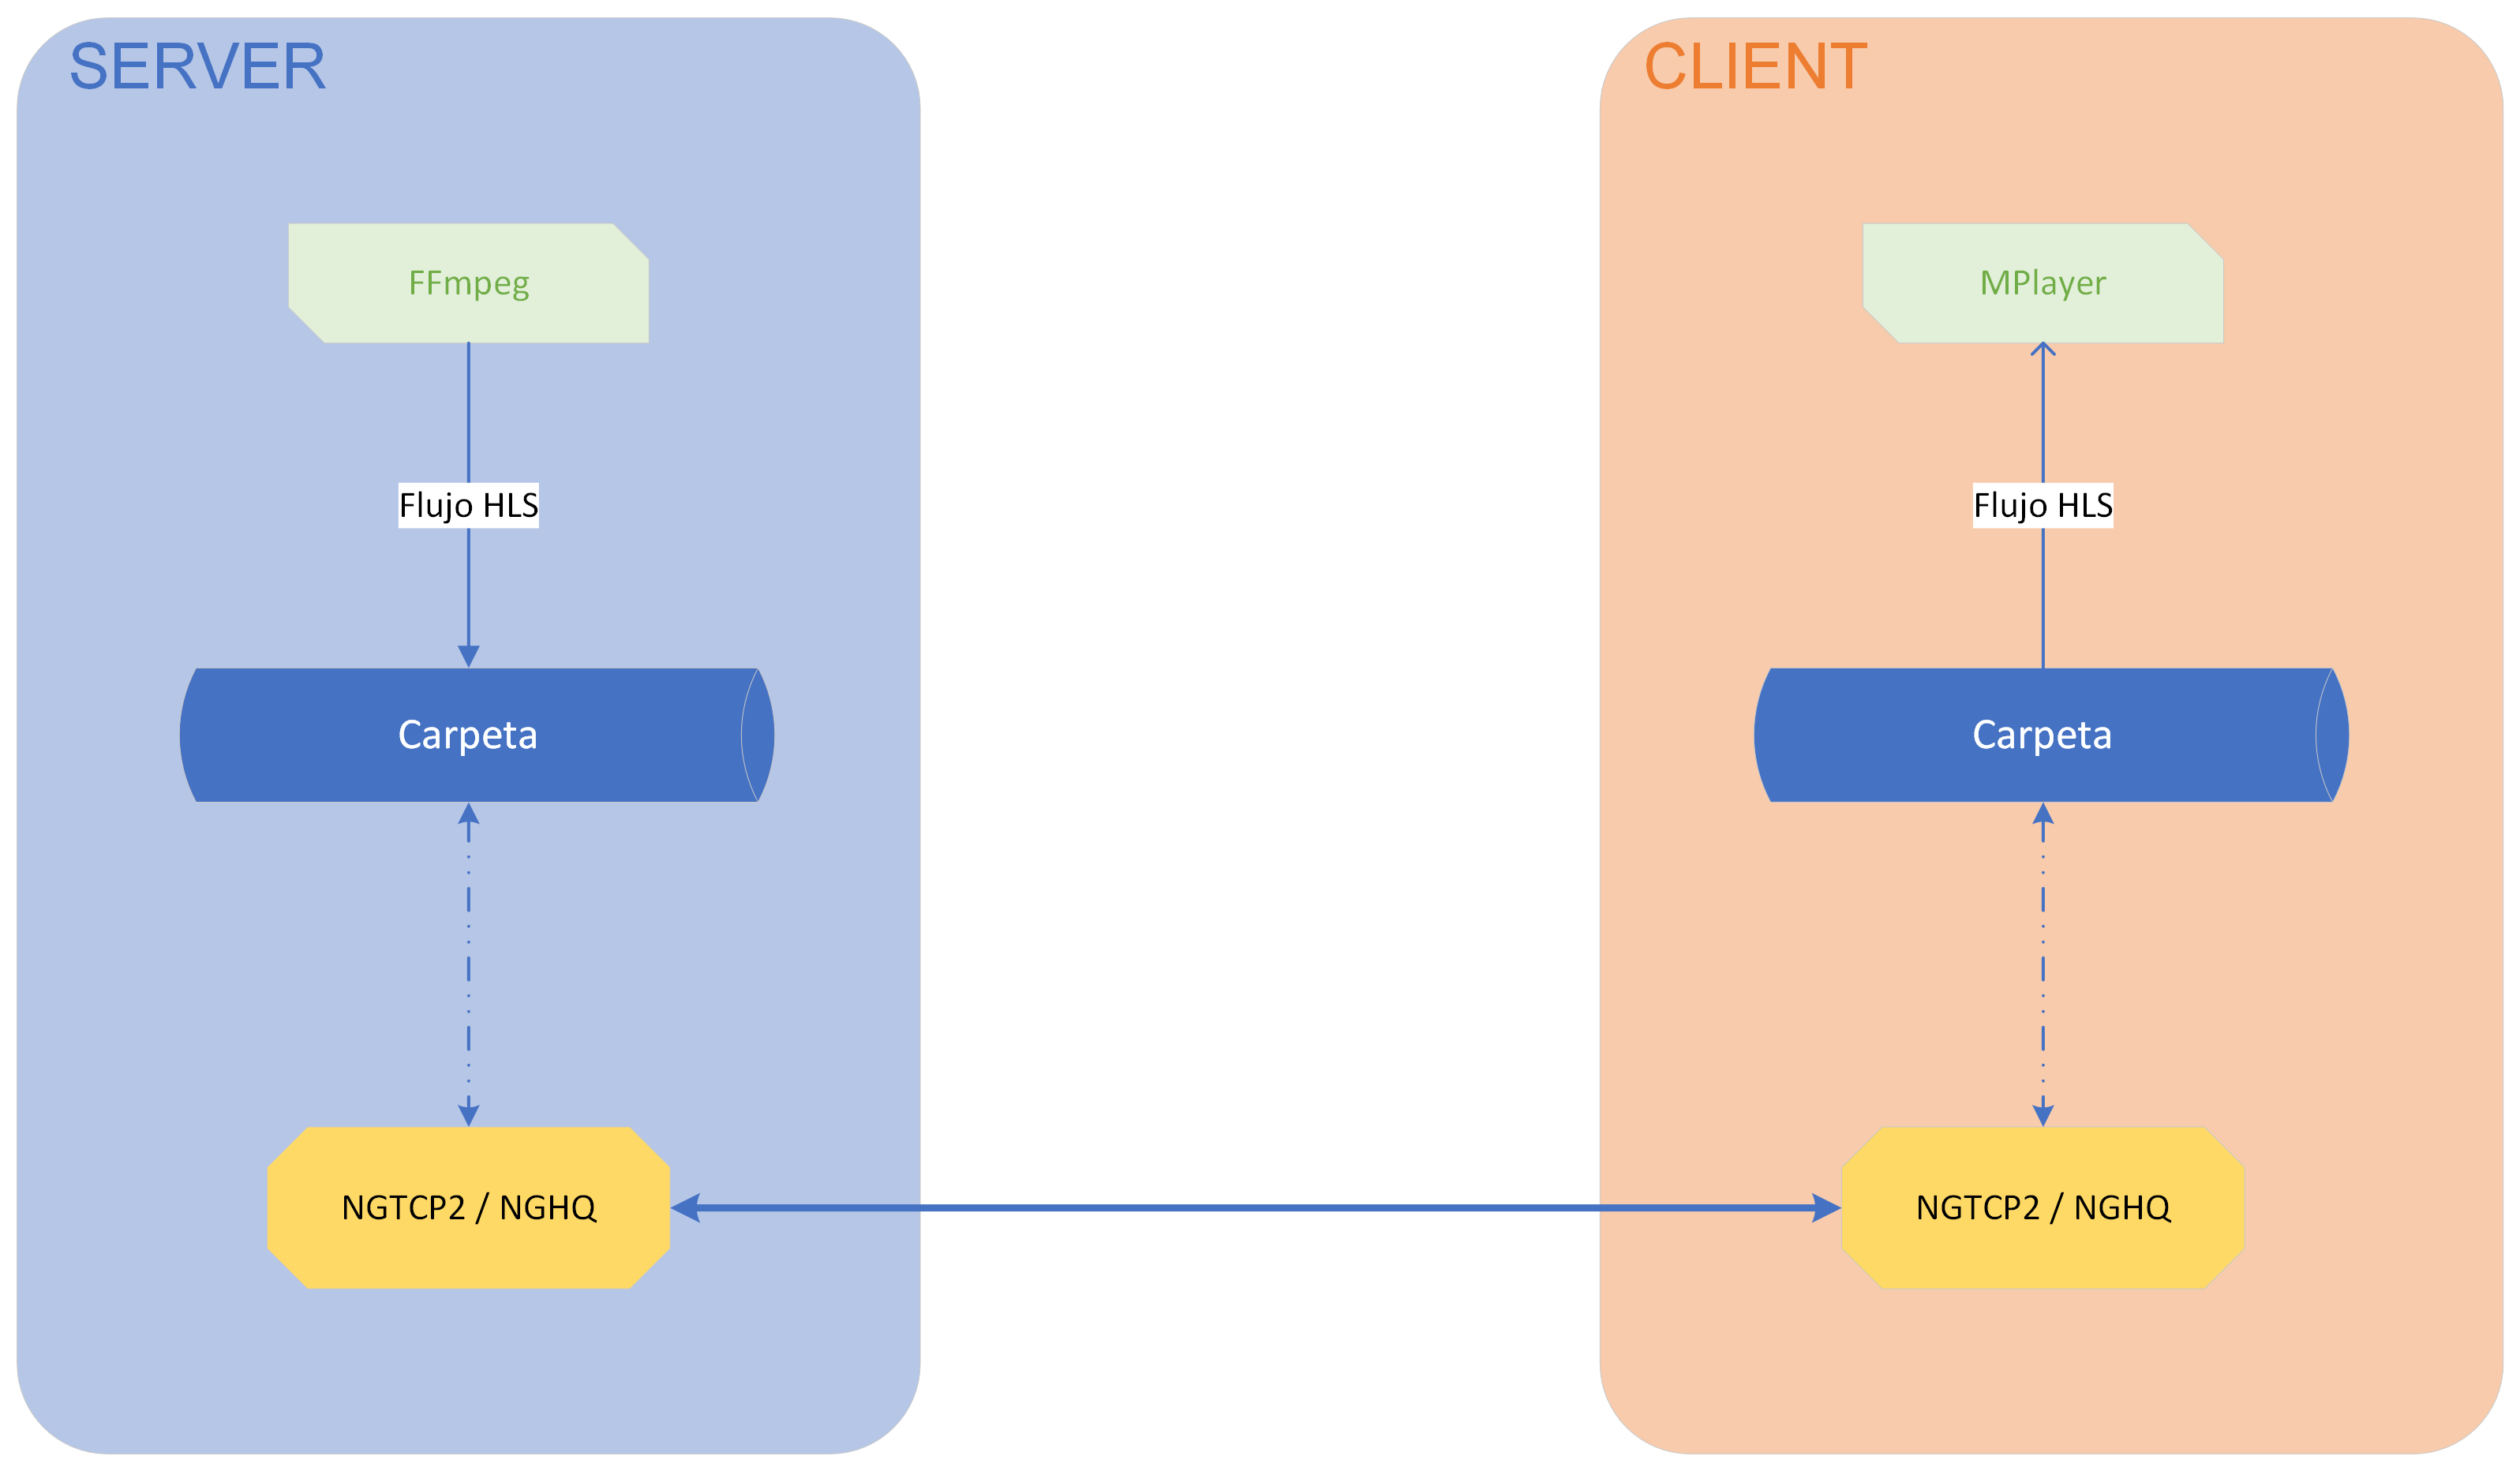
\includegraphics[width=15cm]{img/03_metodologia/system_design.png}
    \end{figure}
}
\subsubsection{Servidor}
{
    Per la banda del servidor, primer de tot es genera un fluxe de contingut amb \textit{ffmpeg} que es guarda en una 
    carpeta. Aquest fluxe és un video en bucle reproduit en temps real codificat en \ac{HLS}\footnote{És l'estàndar de
    codificació de video i audio utilitzat per transmetre contingut en temps real a Internet.}. Una vegada s'ha començat
    a crear el fluxe, aquest es detectat per un script creat en Python que anirà indicant continuament quan s'ha modificat
    l'arxiu de senyalització (.m3u8) i quin és l'últim troç de fluxe de dades creat (.ts).

    En el cas d'unicast, aquest ha de ser demanat pel client (GET) i en el cas de multicast aquest serà enviat directament
    a l'usuari (server Push).
}

\subsubsection{Client}
{
    Per la banda del client, el fluxe creat pel servidor serà rebut (multicast) o demanat (unicast). Aquest s'emmagatzemarà 
    en una carpeta segons vagin arribant. Per poder visualitzar el video live-streaming mentre va arribant es pot inicialitzar
    un reproductor com pot ser Mplayer. S'ha de pensar que l'arxiu de senyalització (.m3u8) està pensat perquè pugui ser modificat
    en temps real (on-the-fly), fet que permet de cara a l'usuari final veure un fluxe continu.
}

\subsection{Metodologia de les proves}
{
    Per una part s'analitza la quantitat de tràfic generat en el cas multicast i en el cas unicast (prova quantitativa) i,
    per altra part, s'analitzarà la qualitat del tràfic rebut mirant el video rebut (prova qualitativa). En el dos casos 
    es faràn les corresponents taules comparatives i comentaris pertinents.

    En el nostre cas, per falta de potència i perquè és un entorn simulat i no un entorn real, no es faràn proves de quin
    és el límit d'usuaris en el servidor unicast. Per la teoria, i pràctica, no té sentit mirar quin és el límit d'usuaris
    en el cas multicast.
}


